\documentclass[a4paper,titlepage,halfparskip,12pt]{scrreprt}

\usepackage[ngerman]{babel, varioref}
\usepackage[utf8]{inputenc}
\usepackage[T1]{fontenc}
\usepackage{graphicx}
\usepackage{fancyhdr}
\usepackage{amsmath}
\usepackage{geometry}
\geometry{a4paper, top=25mm,left=25mm,right=25mm,bottom=25mm, footskip=12mm}
\usepackage{longtable}
\usepackage{setspace}
\usepackage{lmodern}
%blocksatz
\sloppy
%formatierung literaturverzeichnisangabe
\bibliographystyle{unsrt}

%Auflistungen von Punkten
\usepackage{paralist} 
%urls anzeigen
\usepackage{url}

%Codelisting
\usepackage{xcolor}
\definecolor{mygreen}{rgb}{0,0.6,0}
\definecolor{mygray}{rgb}{0.5,0.5,0.5}
\definecolor{mymauve}{rgb}{0.58,0,0.82}
\definecolor{burntorange}{rgb}{0.8, 0.33, 0.0}
\definecolor{cornellred}{rgb}{0.7, 0.11, 0.11}

\usepackage{listingsutf8}
\lstset{
commentstyle=\color{mygreen},
numberstyle=\small\color{black},
stringstyle=\color{mymauve},
emph={square}, 
showstringspaces=false,
flexiblecolumns=false,
tabsize=2,
numbers=left,
numberblanklines=false,
stepnumber=1,
captionpos=b,
numbersep=5pt,
xleftmargin=15pt,
breaklines=true,
inputencoding=utf8,
extendedchars=true,
extendedchars=true,
basicstyle=\ttfamily\footnotesize,
keywordstyle = \bfseries\color{burntorange},
keywordstyle = [2]\bfseries\color{cornellred},
literate=%
    {Ä}{{\"A}}1%
    {Ö}{{\"O}}1%
    {Ü}{{\"U}}1%
    {ä}{{\"a}}1%
    {ö}{{\"o}}1%
    {ü}{{\"u}}1%
    {ß}{{\ss}}1,%
frame=single,
frameround=ffff
}

%meta data
\usepackage[hidelinks]{hyperref}
\urlstyle{same}

%akronymverzeichnis
\usepackage[printonlyused]{acronym}

% titel definieren
\newcommand{\titel}{Entwicklung eines Chatsystems\\auf Basis von XMPP}

%autor definieren
\newcommand{\autor}{Lukas Priester,Oliver Klapper}
\newcommand{\keywords}{\autor,\titel,Studienarbeit}

% Allgemeines für das PDF
\hypersetup{
    pdftitle={\titel},
    pdfauthor={\autor},
    pdfcreator={\autor},
    pdfsubject={\titel},
    pdflang={Deutsch},
    pdfdisplaydoctitle=true,
    pdfkeywords={\keywords},
}

% set distances of chapter headlines in document
\renewcommand*\chapterheadstartvskip{\vspace*{20pt}} % set distance to header
% set distance to text
%\renewcommand*\chapterheadendvskip{%
%  \vspace*{1\baselineskip plus .1\baselineskip minus .167\baselineskip}}


\begin{document}

\begin{table}[h]
\centering
\begin{tabular}{lcr}

\includegraphics[height=3.5cm]{images/dhbw-logo}
\end{tabular}
\end{table}
\bigskip
\bigskip
\begin{center}
\vspace*{12mm} {\LARGE\textbf{\titel}}\\
\vspace*{12mm} {\large\textbf{Studienarbeit}}\\
\vspace*{3mm} {\large\textbf{5. - 6. Semester}}\\
\vspace*{12mm} des Studiengangs Informationstechnik (B.Sc.)\\ an der Dualen Hochschule Baden-Württemberg Stuttgart\\
% \vspace*{3mm} an der Dualen Hochschule Baden-Württemberg\\
\vspace*{12mm} von\\
\vspace*{3mm} {\large\textbf{Lukas Priester, Oliver Klapper}}\\
\vspace*{12mm} \today\\
\end{center}
\vfill
\begin{spacing}{1.5}
\begin{tabbing}
mmmmmmmmmmmmmmmmmmmmmmmmmm \= \kill
\textbf{Bearbeitungszeitraum} \> 01.10.2019 - 01.05.2020\\
\textbf{Matrikelnummer, Kurs} \> 7288057, 4191693 \\
\textbf{Kurs} \> TINF17IN\\
\textbf{Betreuer der Hochschule} \> Alfred Becker\\
\textbf{Gutachter der Hochschule} \> Alfred Becker\\
\end{tabbing}
\end{spacing}
%Seitennummerierung ausschalten
\pagenumbering{gobble}
\newpage

\section*{Selbstständigkeitserklärung}

\bigskip

Ich versichere hiermit, dass ich meine Bachelorarbeit (bzw. Studien- und Projektarbeit) mit dem Thema:

\smallskip

%% eigentlich hier \titel verwenden statt duplicated titel, aber umbruch erzwingt
%% doppeltes ausschreiben des titels
\texttt{Entwicklung eines Chatsystems auf Basis von XMPP}

\smallskip

selbstständig verfasst und keine anderen als die angegebenen Quellen und Hilfsmittel benutzt habe.

\bigskip

Ich versichere zudem, dass die eingereichte elektronische Fassung mit der gedruckten Fassung übereinstimmt.*

\bigskip

\begin{small}

* falls beide Fassungen gefordert sind

\bigskip

\bigskip

\noindent\begin{tabular}{ll}
\makebox[2.5in]{\hrulefill} & \makebox[2.5in]{\hrulefill}\\
Ort, Datum & Unterschrift
\end{tabular}
\end{small}

\newpage

%abstract text
\section*{Abstract}

\newpage

%inhaltsverzeichnis
	% Inhaltsverzeichnis
	\cleardoublepage
	\begin{spacing}{1.1}
		\begingroup
		
			% auskommentieren für Seitenzahlen unter Inhaltsverzeichnis
			\renewcommand*{\chapterpagestyle}{empty}
			\pagestyle{empty}
			
			
			%\setcounter{tocdepth}{1}
			%für die Anzeige von Unterkapiteln im Inhaltsverzeichnis
			\setcounter{tocdepth}{2}
			
			\tableofcontents
			\clearpage
		\endgroup
	\end{spacing}

%% new header/footer settings
\renewcommand{\sectionmark}[1]{\markright{\thesection\ #1}} % make header rightmark
\fancypagestyle{fancyheadlines}{
\pagenumbering{arabic}
\fancyhf{}
\lhead{\slshape\rightmark}
%%\rhead{\slshape\nouppercase{\leftmark}}
\renewcommand{\headrulewidth}{0.4pt}
%\lfoot{\slshape DHBW Stuttgart | Lukas Priester, Oliver Klapper}
\cfoot{\thepage}
\renewcommand{\footrulewidth}{0.4pt}
}

% Redefine the plain page style, show only page number in figure,table,...contents
% and chapter pages
\fancypagestyle{plain}{%
  \fancyhf{}%
  %\lfoot{\slshape DHBW Stuttgart | Lukas Priester, Oliver Klapper}%
  \cfoot{\thepage}
  \renewcommand{\headrulewidth}{0pt}% Line at the header invisible
  \renewcommand{\footrulewidth}{0.4pt}% Line at the footer visible
}


\newpage
\pagenumbering{Roman}


%abkürzungsverzeichnis
\cleardoublepage
\addcontentsline{toc}{chapter}{Abkürzungsverzeichnis}
\chapter*{Abkürzungsverzeichnis}
\begin{acronym}[YTMMM]
\setlength{\itemsep}{-\parsep}

\acro{IMS} {Instant Messaging System}
\acro{XMPP} {Extensible Messaging and Presence Protocol}
\acro{XML} {Extensible Markup Language}
\acro{TCP} {Transmission Control Protocol}
\acro{TLS} {Transport Layer Security}
\acro{MUC} {Multi-User-Chat}
\acro{NLP} {Natural Language Processing}
\acro{MUC} {Multi User Chat}
\acro{ICQ} {I seek you}
\acro{VoIP} {Voice over IP}
\acro{HTML}{HyperText Markup Language}
\end{acronym}

%abbildungsverzeichnis
\cleardoublepage
\addcontentsline{toc}{chapter}{\listfigurename}
\listoffigures
\newpage
%tabellenverzeichnis
\cleardoublepage
\addcontentsline{toc}{chapter}{\listtablename}
\listoftables
\newpage
%listingverzeichnis
\cleardoublepage
\addcontentsline{toc}{chapter}{\lstlistingname}
\lstlistoflistings
\newpage

\begin{onehalfspacing}

%% header and footer settings
\pagestyle{fancyheadlines}

\chapter{Einleitung}
\label{chap:Einleitung}

Social Media (deutsche Übersetzung: \glqq soziale Medien\grqq{}) ist ein aktuelles und wichtiges gesellschaftliches Thema. Die vielfältigen und breitgefächerten Nutzungsmöglichkeiten beeinflussen das Privat- und das Berufsleben \cite{gabriel2017social}. Gabriel und Röhrs definieren Social Media in \cite{gabriel2017social} als die Verwendung digitaler Medien unter Einsatz computergeschützter Technologien, das heißt, von Hardware- und Softwaresystemen. Sie definieren den Nutzen von Social Media darin, dass Menschen Informationen suchen, erstellen, verteilen und austauschen können. Es gibt eine große Anzahl an unterschiedlichen Definitionen von Social Media. Nach Liu Yinyuan ist Social Media längst wichtiger Bestandteil des Unternehmensmarketings in Deutschland. In seinem Werk \glqq Social Media in China\grqq{} \cite{liu2016social} beschreibt er, dass in Unternehmen nicht mehr über die grundsätzliche Frage debattiert wird, ob Social Media für das Unternehmensmarketing eingesetzt werden soll, sondern wo und wie der Einsatz zielgerichtet erfolgen kann. Heutige Unternehmen sind gekennzeichnet von computergestützten Anwendungssystemen, die in allen Funktionsbereichen zur Planung, Steuerung und Kontrolle der Geschäftsprozesse und zu ihrer Verwaltung eingesetzt werden. Sie setzen dieses System in der B2B-Kommunikation (Business-To-Business-Kommunikation) ein. Immer wichtiger werden \textbf{\ac{IMS}}, wie zum Beispiel Whatsapp, Telegram, iMessage und Jabber, die dazu dienen intern Informationen schnell im Unternehmen zu verbreiten, hoch verfügbar zu machen und um Geschäftsprozesse standortunabhängig steuern zu können \cite{gabriel2017social}. Zusätzlich werden \textbf{Instant Messaging Systeme} auch zur externen Kommunikation benutzt. Nach Gabriel und Röhrs ist es möglich, dass mehrere Unternehmen mit Hilfe von innovativen Kommunikationstechniken zur Erreichung eines gemeinsamen Ziels besser kooperieren können. Außerdem ist die schnelle und direkte Kontaktaufnahme von Kunden über ein Messaging System zum Support eines Unternehmens eine einfache und schnelle Möglichkeit, Fragen zum Produkt ohne langes Warten in der Hotline zu stellen. Nach \cite{b2bmehner} werden Nachrichten von \textbf{Instant Message Systemen} im Gegensatz zu einer E-Mail in Echtzeit übertragen und dem Empfänger direkt zugestellt. Laut einer Statistik von \textbf{statista} benutzen 1,5 Milliarden Nutzer in Deutschland pro WhatsApp pro Monat \cite{statistaIMS}. Der Anteil der Nutzer von Whatsapp in Deutschland beträgt 75 Prozent an der Gesamtbevölkerung \cite{statistaIMS}. Die Statistik zeigt, dass \textbf{Instant Messaging Systeme} eine Möglichkeit in der Zukunft darstellen Kunden direkter anzusprechen oder Support zu gewährleisten. Zusätzlich zu Nachrichtendiensten werden künstliche Intelligenzen und Algorithmen benötigt, die Nutzer unterstützen oder gesammelte Daten von Benutzern charakterisieren oder interpretieren können. Algorithmen werden verwendet, um zum Beispiel die emotionale Befindlichkeit anhand eines Text einzuordnen, um Suizid-Gedanken frühzeitig zu erkennen \cite{stasytisIME}. Ein weiteres Anwendungsszenario sind Text-to-Speech (deutsche Übersetzung: Text-zu-Sprache) Funktionalitäten, bei denen gesprochene Worte des Nutzers durch Algorithmen in Text umgewandelt werden, sodass ein Nutzer die Nachricht nicht mehr aktiv eintippen muss. Eine wichtige Teilaufgabe ist die Recherche und das Versehen von datenschutzrechtlichen Aspekten, die bei der Datenspeicherung und der Implementierung von \textbf{Instant Messaging Systemen} bestehen.

\section{Aufgabenstellung}
\label{sec:Aufgabenstellung}

Die konkrete Aufgabe ist es, einen Chatserver auf Basis des \textbf{\ac{XMPP}} in Betrieb zu nehmen über den sich mehrere Chat-Clients authentifizieren und verschlüsselt Nachrichten austauschen können. Durch eine gründliche Recherche soll eruiert werden, welcher Chatserver sich hierfür eignet und warum dieser Chatserver für das Projekt verwendet wird. Der Nachrichtenaustausch soll Ende-zu-Ende verschlüsselt erfolgen. Eine wichtige Teilaufgabe ist, dass die Software Gruppenchats verschlüsselt unterstützt. Eine Zustellung der Nachrichten in Echtzeit soll implementiert werden. Benutzer sollen Nachrichten über eine Web-Oberfläche eingeben und empfangen können. Es soll ein Prototyp eines Machine Learning Algorithmus der Kategorie \textbf{\ac{NLP}} implementiert werden und in die Web-Oberlfäche integriert werden. Eine wichtige Aufgabe ist, dass das gesamte Chatsystem datenschutzfreundlich implementiert und programmiert wird.

\section{Ziele der Arbeit}
\label{sec:Ziele}

Die Ziele der Arbeit sind es, eine geeignete Netzwerkumgebung und einen lauffähigen Chatserver auf Basis von \ac{XMPP} in Betrieb zu nehmen. Es sollen tiefe Kenntnisse und Erfahrungen mit dem Umgang des \ac{XMPP} Protokolls gesammelt werden und sich mit dem Aufbau des Nachrichtenprotokolls auseinandergesetzt werden. Außerdem sollen sich mit der Arbeitsweise und den Grundlagen von \textbf{Instant Messaging Systemen} und der Nachrichtenübertragung in Echtzeit vertraut gemacht werden. Es soll ein funktionsfähiger Prototyp einer WebUI entstehen, der einen \ac{MUC} unterstützt und über den Chatserver Nachrichten verschlüsselt versendet und empfängt. Durch Recherche und praktische Entwicklungen soll das Fachwissen in der Programmiersprache \textbf{Python} vertieft werden. Zusätzlich sollen Fähigkeiten im Bereich \textbf{Machine Learning} erlernt werden und ein lauffähiger Prototyp eines \ac{NLP}-Models in die Weboberfläche integriert werden. Das letzte Ziel beinhaltet, Kenntnisse im Bereich des Datenschutzes bei Chatapplikationen zu erarbeiten und den Chatserver datenschutzfreundlich zu konfigurieren.

\section{Stand der Technik}
\label{sec:StandDerTechnik}

\textbf{Instant Messaging Systeme} existieren in der heutigen Form seit Ende der 1990er Jahre, ausgehend von einer Öffnung des Internets für einen größeren Nutzerkreis außerhalb von Forschungsinstitutionen. Das erste \ac{IMS}, welches eine größere Verbreitung fand, war \textbf{\ac{ICQ}} der Firma Mirabilis, welches Benutzern ermöglicht in einer grafischen Oberfläche Nachrichten untereinander oder in Chatrooms auszutauschen \cite{ICQ}. Die Systeme werden in unterschiedlichen Ausprägungen stets weiterentwickelt. Es kommen zur grundlegenden Funktion des Nachrichtenaustauschs weitere Features, wie Dateiübertragung, \textbf{\ac{VoIP}}, Video over IP, \textbf{Ende-zu-Ende-Verschlüsselung} oder Sprachnachrichten hinzu \cite{gross2007}. 
Weitere typische Funktionen sind die Möglichkeit des Logins mit Passwort und die Angabe der Verfügbarkeit oder die Übermittlung seines Standorts an andere Benutzer. Die Ansprüche an Funktionalitäten von Chatsystemen und der Echtzeitübertragung wachsen stetig weiter und es ist zu erwarten, dass in den kommenden Jahren der Fortschritt die Echtzeitübertragung und die Funktionalitäten von \textbf{Instant-Messaging-Systeme} verbessern wird. Um einen Beitrag zur Steigerung der Präsenz und der Funktionalitäten zu leisten, soll ein Chatsystem gebaut werden, dass den Anforderungen bisheriger Chatsysteme entspricht. Das Chatsystem soll die Datenschutzbestimmung erfüllen und Benutzerdaten nur speichern, wenn dies für die Bereitstellung des Dienstes nötig ist.\cite{anastasiaIMS}
\newpage

\chapter{Datenschutzrechtliche Aspekte}
\label{chap:Datenschutz}

\newpage

\chapter{Anforderungen}
\label{Anforderungen}

\newpage

\chapter{Theoretische Grundlagen}
\label{chap:Theorie}

\section{Funktionsweise von Instant-Messaging-Systemen}
\label{sec:IMSFunktion}

Verschiedene \ac{IMS} besitzen ähnliche Funktionsweisen. Möchte ein Bentzer einen \ac{IMS} nutzen, muss dieser eine bestimmte Software installieren. Diese Software wird als \textbf{Instant-Messaging-Client (IM-Client} bezeichnet. Der Benutzer muss sich an einem Authentifikationsserver registrieren. Es wird ein Benutzerprofil angelegt, welches aus aus einem Benutzernamen (User ID) und einem Passwort (Pre-Shared-Key) besteht. Diese Daten werden beim Login des Benutzers vom \ac{IMS} abgefragt. Ein Benutzerprofil kann weitere personenbezogenen Daten bestehen, wie zum Beispiel, Wohnort, Geschlecht und Geburtsdatum. Die Anzahl der Server für die Authentifizierung und der Bereitstellung des Dienstes variiert je nach der Anforderung an Verfügbarkeit und Anzahl der zu erwartenden Nutzer des \ac{IMS}. Die horizontale Skalierung von Servern und Diensten unterliegt allein dem Betreiber dieser Systeme, häufig finden sich jedoch Cluster-Systeme mit intelligenter Lastverteilung (Load-Balancing). \autoref{img:StrukturIMS} zeigt den allgemeinen Aufbau eines \ac{IMS}. In der Abbildung wird eine horizontale oder vertikale Skalierung des \ac{IMS} vernachlässigt. Der Authentifikationsserver symbolisiert einen oder mehrere Server.\cite{anastasiaIMS}

\begin{figure}[h]
	\centering
	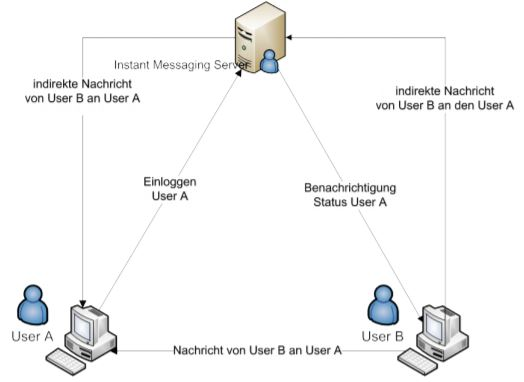
\includegraphics{images/GrundlegendeStrukturIMS}
	\caption{Allgemeine Struktur eines Instant-Messaging-Systems}
	\label{img:StrukturIMS}
\end{figure}

Hat sich der Benutzer mit seinen Login-Daten erfolgreich gegenüber dem Authentifikationsserver authentifiziert, kann er andere, bereits registrierte, Benutzer kontaktieren. Die Verbindungsinformationen wie zum Beispiel IP-Adresse, die dem Client lokal zugewiesene Portnummer und die Kontaktliste (Freunde des Benutzers) werden an den Präsenzserver übermittelt. Dieser ist abhängig von der Implementierungsform ein Teil des \textbf{IM-Servers} oder ein eigenständiger Server. Der Präsenzserver überprüft, welche Benutzer aus der Kontaktliste verfügbar und angemeldet sind. Der Server sendet dem Benutzer die Ergebnisse der Statusüberprüfung zurück. Ist einer der gewünschten Benutzer \glqq online\grqq (verfügbar) kann durch die Auswahl der entsprechenden Kennung eine Verbindung aufgebaut werden und der Nachrichtenaustausch kann beginnen. Dies ist möglich, weil der Server dem Sender die IP-Adresse und die Ziel-Portnummer des Kommunikationspartners übermittelt. Die Nachrichten werden direkt zwischen den Clients übertragen oder über den Server zwischen den Kommunikationspartnern übermittelt. Die Art der Übertragung ist von System zu System je nach Realisierung unterschiedlich. Der Kommunikationspfad ist abhängig von der Architektur und dem verwendeten Protokoll. Eine Nachricht kann zentral über den Server vermittelt werden (vgl. \autoref{img:StrukturIMS}-indirekte Nachricht) oder nach dem Peer-to-Peer-Prinzip (vgl. \autoref{img:StrukturIMS}-direkte Nachricht) erfolgen. 

\section{XMPP-Extensible Messaging and Presence Protocol}
\label{sec:XMPP}
\ac{XMPP} bedeutet \textbf{Extensible Messaging and Presence Protocol}. Übersetzt man dies detailliert ins deutsche so ergibt sich ein erweiterbares Nachrichten- und Anwesenheitsprotokoll. Eine Definition die \ac{XMPP} sehr gut beschreibt. \ac{XMPP} basiert auf \ac{XML}, welches eine Markup Sprache darstellt. Das Ziel von \ac{XMPP} war ein Protokoll für das Instant Messaging zu entwickeln. Laut dem RFC6120 lässt sich mittels \ac{XMPP} Daten zwischen zwei oder mehreren Netzwerkeinheiten nahezu in Echtzeit austauschen, welches als Vorteil für Sofortnachrichten bezeichnet werden kann. Diesbezüglich nutzt es das Internet und erlaubt den Usern Sofortnachrichten an andere Anwender innerhalb des Internets zu schicken. \ac{XMPP} lässt sich in viele verschiedene Funktionen aufteilen, weshalb der grundlegende Zweck ein anderes Ziel verfolgt. Im einfachsten Sinne ist die Idee von \ac{XMPP} den Austausch von kleinen Teilen strukturierter Daten (\glqq \ac{XML} stanzas\grqq) zwischen einem oder mehreren Netzwerkteilnehmern zu ermöglichen. Primär wird \ac{XMPP} mithilfe einer Client-Server-Architektur implementiert, bei der sich ein Client mit einem Server verbindet, um mit anderen Teilnehmern Daten auszutauschen. Anderseits kann es als Protokoll auch zwischen Servern fungieren. Daraus resultiert der Vorteil nahezu unabhängig von Betriebssystemen und Browsern zu sein. Wird die Client-Server-Architektur implementiert, so ist in der Regel der Ablauf definiert durch folgende Schritte: \cite{RFC6120} 
\begin{enumerate}
	\item Bestimmen der IP-Adresse und des Ports zu dem sich verbunden werden soll 
	\item Eine \ac{TCP} Verbindung öffnen/aufbauen
	\item Öffnen eines \ac{XML}-Streams über \ac{TCP}
	\item Optional: Verwendung von \ac{TLS} für die Verschlüsselung
	\item Verwendung des SASLs Frameworks für die Authentifizierung
	\item Eine Ressource an den \ac{XML} stream anbinden
	\item Austausch unbegrenzter \glqq \ac{XML} stanzas\grqq ()=> kleine Teile strukturierter Daten) mit anderen Netzwerkteilnehmern
	\item Schließen des \ac{XML} streams
	\item Schließen der \ac{TCP} Verbindung
\end{enumerate}
Die folgende \autoref{img:XMPPcommunication} zeigt den Start einer Kommunikation, wie im genannten Ablauf dargestellt, über \ac{XMPP} und den \ac{XML}-streams.

\begin{figure}[h]
	\centering
	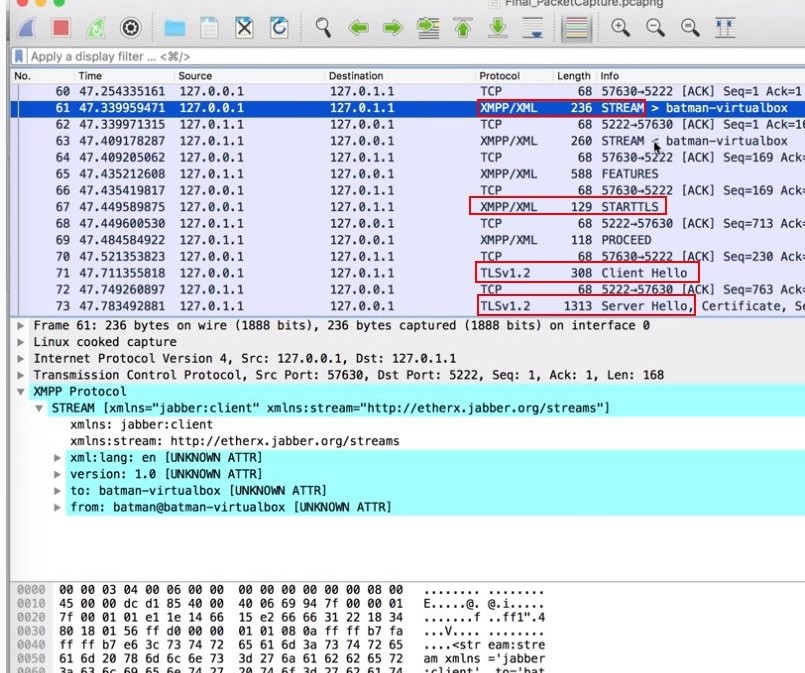
\includegraphics[width=\textwidth]{images/XML_Wireshark}
	\caption{Kommunikationsaufbau des \ac{XMPP}-Protokolls}
	\label{img:XMPPcommunication}
\end{figure} 
\newpage
Für den Austausch von Daten gibt es zwei elementare Konzepte. Zum einen die \ac{XML}-Streams und die \ac{XML}-Stanzas. Diese zwei Konzepte werden definiert um das Verständnis des Datenaustauschs, wie es im obigen Ablauf definiert ist, zu erlangen. Bei dem Austausch der Daten mittels \ac{XML} streams wird von einem Container zwischen den Teilnehmern gesprochen. Der \ac{XML} stream ist durch den \glqq stream header\grqq (z.B. \ac{XML} <stream>) und dem Ende des streams, dargestellt durch \ac{XML} </streams>, eindeutig definiert. Die Anzahl der austauschbaren \ac{XML} Elemente ist unbegrenzt und durch die Lebensdauer des streams definiert. Das \ac{XML} stanza wird nun als diskrete semantische Einheit strukturierter Daten, das von einem Teilnehmer zu einem anderen über den \ac{XML} stream gesendet wird bezeichnet. Das \ac{XML} stanza ist ein direktes Kind-Element des streams. Ein stanza kann wiederum selbst Kind-Elemente enthalten, das den \ac{XML} stream definiert. Im Kern fungiert der \ac{XML} stream wie eine Hülle um alle \ac{XML} stanzas, die während einer Session versendet werden. Ein Aufbau kann wie in der folgenden \autoref{img:StrukturXMLstream} repräsentiert werden. \cite{RFC6120Sec4}
\begin{figure}[h]
	\centering
	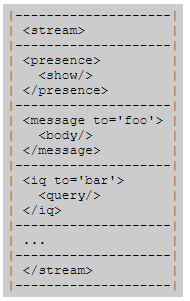
\includegraphics[scale=1.2]{images/XML_Stream}
	\caption{Allgemeine Struktur eines XML streams}
	\label{img:StrukturXMLstream}
\end{figure}
\newpage


\section{Python}
\label{sec:Python}
\newpage

\section{Ejabberd}
\label{sec:ejabberd}
Ejabberd ist einer der bekanntesten freien \ac{XMPP}-Server auf der Welt und kann in vielerlei Hinsicht verwendet werden. Sowohl Großprojekte als auch kleine Instanzen machen sich die Eigenschaften von ejabberd zum Vorteil. Der Start von ejabberd ist dem Jahr 2002 zuzuordnen. Ejabberd ist eine Abkürzung und steht für \glqq Erlang Jabber Daemon\grqq. Wie die Definition zeigt bezieht sich ejabberd auf die Programmiersprache Erlang. Grund hierfür ist, dass die ejabberd Software in Erlang geschrieben ist. Seit dem Start wurde es von Grund auf für die Unternehmensbereitstellung entwickelt, vor allem mit dem Ziel robust zu sein. Aufgrund davon, dass der Fokus auf die Unternehmen lag, war es wichtig die Fehleranfälligkeit von ejabberd zu minimieren. Ein Vorteil der sich bis zum heutigen Zeitpunkt bewahrt hat. Außerdem kann ejabberd die Ressourcen mehrerer geclusterter Systeme nutzen. Des Weiteren besitzt ejabberd die Eigenschaft der Skalierbarkeit, indem die Kapazitäten mit wenig Aufwand erhöht werden kann. Während der Entstehungsphase war das \ac{XMPP}-Protokoll, welches in \autoref{sec:XMPP} beschrieben wird, noch unter dem Namen Jabber bekannt. Ejabberd kann verschieden benutzt werden. Im Fall der Studienarbeit wird die Community Edition von ejabberd benutzt, welche als open source zur Verfügung steht. Neben der Community Edition gibt es auch noch Möglichkeiten einer Business Edition, welches vor allem für die großen Unternehmen mit besserem Support rund um die Uhr und größeren Funktionen konzeptioniert ist. Die Architektur eines ejabberd services erweitert die Kernfunktionen von \ac{XMPP}, welches das Senden von Nachrichten ist, um Faktoren wie die Skalierbarkeit, Konfigurierbarkeit und Fehlertoleranz. Außerdem gilt die Architektur von ejabberd als Modular. Das bedeutet, dass es an den Zweck eines Projektes angepasst werden kann. Die Modularität bringt bspw. Funktionen wie Gruppenchat mit ein. Aufgrund der großen Anzahl an Modulen werden lediglich die Module, die für das Projekt relevant sind aufgelistet.
Relevante Funktionen:
\begin{itemize}
	\item Einzelchat
	\item Gruppenchat (auch als Multi-User-Chat (\ac{MUC}) bezeichnet)
	\item Offline Nachrichten 
	\item Web-Unterstützung
	\item Nachrichtenübermittlungsbestätigung
\end{itemize}
Eine wichtige Eigenschaft ist das Authentifizieren von Nutzern, welches ebenfalls von ejabberd unterstützt wird. Dafür kann ejabberd sowohl mit einer internen, als auch mit einer externen Datenbank zusammenarbeiten. Aufgrund der genannten Eigenschaften und Funktionen von ejabberd, werden eine Vielzahl an mögliche Anwendungsgebieten abgedeckt. Während für viele kleine Projekte die interne Datenbank Mnesia ausreichend ist, wird im Rahmen der Studienarbeit mit einer externen Datenbank gearbeitet.\cite{EjabberdDoc}

\section{Chatserver}
\label{sec:Chatserver}

\begin{lstlisting}[language=Python,caption=Example Listing Python,label={lst:Example}]
"""The first step is to create an SMTP object, each object is used for connection 
with one server."""

import smtplib
server = smtplib.SMTP('smtp.gmail.com', 587)

#Next, log in to the server
server.login("youremailusername", "password")

#Send the mail
msg = "
Hello!" # The /n separates the message from the headers
server.sendmail("you@gmail.com", "target@example.com", msg)
\end{lstlisting}


\section{Datenbank}
\label{sec:Datenbank}

\newpage

\chapter{Umsetzung und Implementierung}
\label{chap:Umsetzung}

\section{Vorbereitung}
\label{sec:Vorbereitung}

\section{Implementierung des Chatservers ejabberd}
\label{sec:ChatserverEntwicklung}

\subsection{Anbindung des Chatservers}
\label{subsec:Anbindung}

\subsection{Security}
\label{subsec:Security}

\subsection{Konfiguration von ejabberd}
\label{subsec:Konfiguration}

\newpage

\section{Entwicklung des Chat-Clients}
\label{sec:ClientEntwicklung}

\ac{HTML}

\subsection{Entwicklung der GUI}
\label{subsec:EntwicklungGUI}

\subsection{Implemintierung des Backends}
\label{subsec:Backend}

\newpage

\chapter{Datenanalyse}
\label{chap:Datenanalyse}

\newpage

\chapter{Ergebnis}
\label{chap:Ergebnis}

\newpage

\chapter{Fazit}
\label{chap:Fazit}


\end{onehalfspacing}
\newpage

\bibliography{Literatur}
\newpage
%setze Anhang mit appendix
%addpart, sodass Anhang im Inhaltsverzeichnis ohne Buchstaben auftaucht
\appendix
\addpart{Anhang}

\end{document}